\documentclass[12pt,a4paper]{article}
\usepackage[margin=0.8in]{geometry}
\usepackage{tikz}
\usetikzlibrary{arrows.meta,positioning}
\pagestyle{empty}
\begin{document}
\section*{Group B: interim selection accounting}
Preliminary recommendations are not final screened exclusions. Final eligibility and unique studies remain pending.
\begin{center}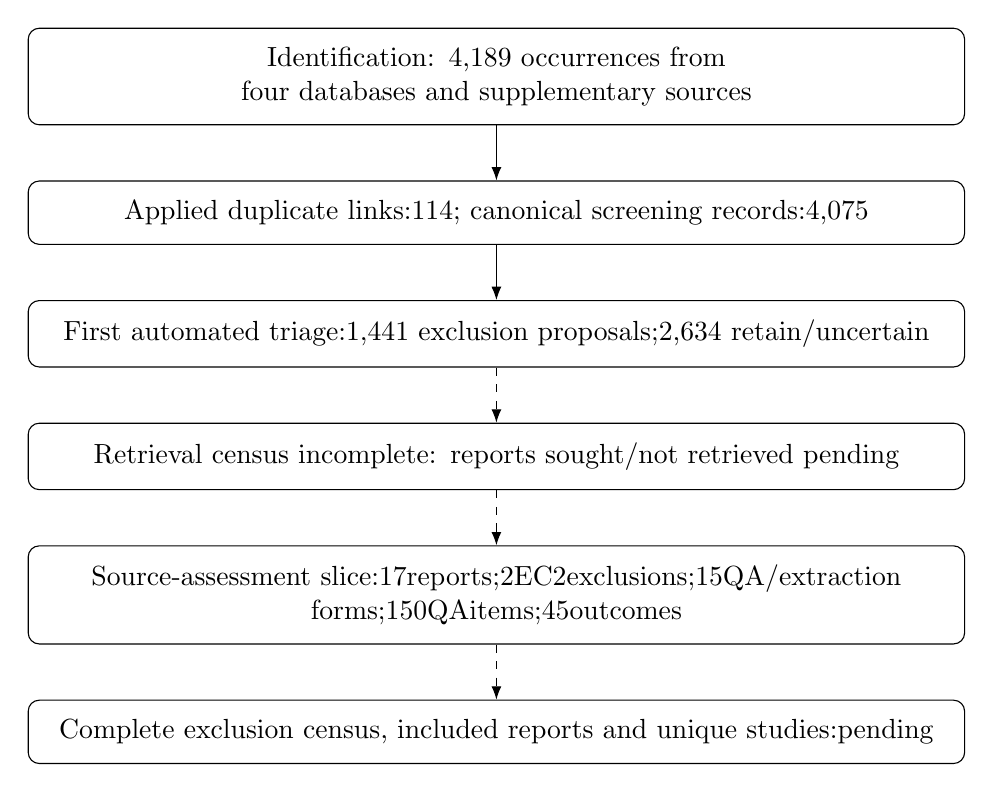
\begin{tikzpicture}[node distance=7mm,box/.style={draw,rounded corners,align=center,text width=11.4cm,inner sep=7pt},>=Latex]
\node[box](a){Identification: 4,189 occurrences from four databases and supplementary sources};
\node[box,below=of a](b){Applied duplicate links:114; canonical screening records:4,075};
\node[box,below=of b](c){First automated triage:1,441 exclusion proposals;2,634 retain/uncertain};
\node[box,below=of c](d){Retrieval census incomplete: reports sought/not retrieved pending};
\node[box,below=of d](e){Source-assessment slice:17reports;2EC2exclusions;15QA/extraction forms;150QAitems;45outcomes};
\node[box,below=of e](f){Complete exclusion census, included reports and unique studies:pending};
\draw[->](a)--(b);\draw[->](b)--(c);\draw[dashed,->](c)--(d);\draw[dashed,->](d)--(e);\draw[dashed,->](e)--(f);
\end{tikzpicture}\end{center}
\end{document}
